%%%%%%%%%%%%%%%%%%%%%%%%%%%%%%%%%%%%%%%%%%%%%%%%%%%%%%%%%%%%%%%%%%%%%%%%%%%%%%%%
%2345678901234567890123456789012345678901234567890123456789012345678901234567890
%        1         2         3         4         5         6         7         8

\documentclass[letterpaper, 10 pt, conference]{ieeeconf}  % Comment this line out if you need a4paper

%\documentclass[a4paper, 10pt, conference]{ieeeconf}      % Use this line for a4 paper

\IEEEoverridecommandlockouts                              % This command is only needed if 
                                                          % you want to use the \thanks command

\overrideIEEEmargins                                      % Needed to meet printer requirements.

% See the \addtolength command later in the file to balance the column lengths
% on the last page of the document

% The following packages can be found on http:\\www.ctan.org
%\usepackage{graphics} % for pdf, bitmapped graphics files
%\usepackage{epsfig} % for postscript graphics files
%\usepackage{mathptmx} % assumes new font selection scheme installed
%\usepackage{times} % assumes new font selection scheme installed
\usepackage{amsmath} % assumes amsmath package installed
\usepackage{amssymb}  % assumes amsmath package installed
\usepackage{graphicx}
\usepackage[hidelinks]{hyperref}
\usepackage{placeins}
\usepackage[font=footnotesize]{caption}

\newcommand{\bolds}[1]{{\bf #1}} 
\newcommand*{\Scale}[2][4]{\scalebox{#1}{$#2$}}%
\newenvironment{bottompar}{\par\vspace*{\fill}}{\clearpage}

\title{\LARGE \bf
Implementing Hill Climbing with a Spiking Neural Network*
}


\author{Aaron Russell Voelker$^{1}$% <-this % stops a space
\thanks{*Funding for this work was provided by the National Science and Engineering Research Council of Canada}% <-this % stops a space
\thanks{$^{1}$Aaron Russell Voelker is with the Centre for Theoretical Neuroscience, University of Waterloo, ON, N2L 3G1
        {\tt\small arvoelke@uwaterloo.ca}}%
}

\begin{document}



\maketitle
\thispagestyle{empty}
\pagestyle{empty}


%%%%%%%%%%%%%%%%%%%%%%%%%%%%%%%%%%%%%%%%%%%%%%%%%%%%%%%%%%%%%%%%%%%%%%%%%%%%%%%%
\begin{abstract}

The hill climbing algorithm, a technique for optimizing some function, is implemented using a neural network of spiking neurons. This network consists of three neural populations, encoding the position, velocity, and acceleration of an input vector. The vector is continuously evaluated by the function to generate an error signal with respect to the current velocity. This paper's main contribution is a heuristic which combines the error with oscillatory perturbations across an arbitrary basis, in order to drive the input in an exploratory manner. We show that this network converges to local optima for a number of test functions, and has interesting qualitative properties stemming from the choice of perturbations. This suggests that a similar heuristic may find use in non-neural implementations.

\end{abstract}


%%%%%%%%%%%%%%%%%%%%%%%%%%%%%%%%%%%%%%%%%%%%%%%%%%%%%%%%%%%%%%%%%%%%%%%%%%%%%%%%
\section{Introduction}

The hill climbing algorithm is an optimization procedure that searches for the minimum of some function, $f$, by evaluating candidates in the local neighbourhood of a vector $\bolds{x}$, so as to greedily obtain incrementally better solutions \cite{russell1995modern}.

Hill climbing has been used to optimize the parameters of Bayesian networks \cite{bayesianstructure} and the connection weights of neural networks \cite{chalup1999study}, but to the author's knowledge no work has yet attempted the reverse: implement the hill climbing algorithm using a neural network.

Within this setting, the function $f$ represents some computation performed by a region of the brain, and the input is given by the spiking activity of a separate population of neurons. Since this input vector is a continuous time-varying signal, it is denoted $\bolds{x}(t)$ to emphasize the importance of time. The goal is to drive $\bolds{x}(t)$ so that $f(\bolds{x}(t))$ is eventually minimized. 

Given these constraints, we do not have the freedom to simply evaluate a discrete set of candidates before updating the current solution, as is the case for a conventional hill climbing implementation. Rather, the network makes use of continuous feedback to dynamically update the current solution based on the function's rate of change with respect to the input's velocity, $\bolds{x}'(t)$. 

This is a considerable disadvantage, since the available information is limited to a sample of the function's gradient along the chosen trajectory. However, this same constraint is faced by stochastic hill climbing, which evaluates only a single randomly chosen neighbour, and thus has the potential benefit of fewer function evaluations. Stochastic hill climbing has also been used to solve problems in reinforcement learning \cite{kimura1995reinforcement}, and so it seems appropriate to adopt a similar approach when using continuous feedback.

The algorithm is carried out in the simulation of a spiking neural network built using the principles of the Neural Engineering Framework (NEF) \cite{eliasmith2003neural}. These methods have been used to model tasks ranging from reinforcement learning to motor control, with quantitative comparisons to both behavioural and spiking data \cite{Rasmussen2014b, dewolf2011, eliasmith2012}.

By constraining the model using NEF principles, this work may shed light on what strategies are feasible for the brain during cognitive tasks that can be formulated as a local search problem.

% Specific applications, as well as evidence that these strategies exist in nature, are discussed in closing. ?
%\cite{hinson1983matching} evidence of hillclimbing strategies in bird behaviour

First, the model is described mathematically in terms of vectors and transformations of these vectors. Second, a brief overview is given on how the NEF compiles this description into a spiking neural network. Third, results are given for several test functions. Last, we discuss how this approach may inform a novel non-neural implementation, as well as some limitations and future directions.

\section{Model} \label{sec-model}

The model contains three neural populations encoding the position, velocity, and acceleration of the function's $d$-dimensional input vector, denoted $\bolds{x}(t)$, $\bolds{v}(t)$, and $\bolds{a}(t)$, respectively. Position is recurrently connected to integrate velocity (so that $\bolds{v}(t) = \bolds{x}'(t)$), and similarly velocity integrates acceleration ($\bolds{a}(t) = \bolds{v}'(t)$). 

The signal $\bolds{x}(t)$ is continuously evaluated by some function $f : \mathbb{R}^d \rightarrow \mathbb{R}$, and crucially the implementation of this function is hidden from the rest of the system. $dy$ tracks the function's rate of change across a $10$ms interval. Similarly, the change in $\bolds{x}(t)$, denoted $d\bolds{x}$, is computed over a $10$ms interval. 

Intuitively, the quantity $(-dy)d\bolds{x}$ represents what ``force'' (i.e. acceleration) should be applied to $\bolds{x}$ to push it in a direction that will decrease error. If the current velocity is causing the error to decrease, then a force is applied in the direction of the velocity. Conversely, if the error is increasing, then a force is applied in the opposite direction, causing the input to reverse direction.

\begin{figure}[ht]
  \centering
  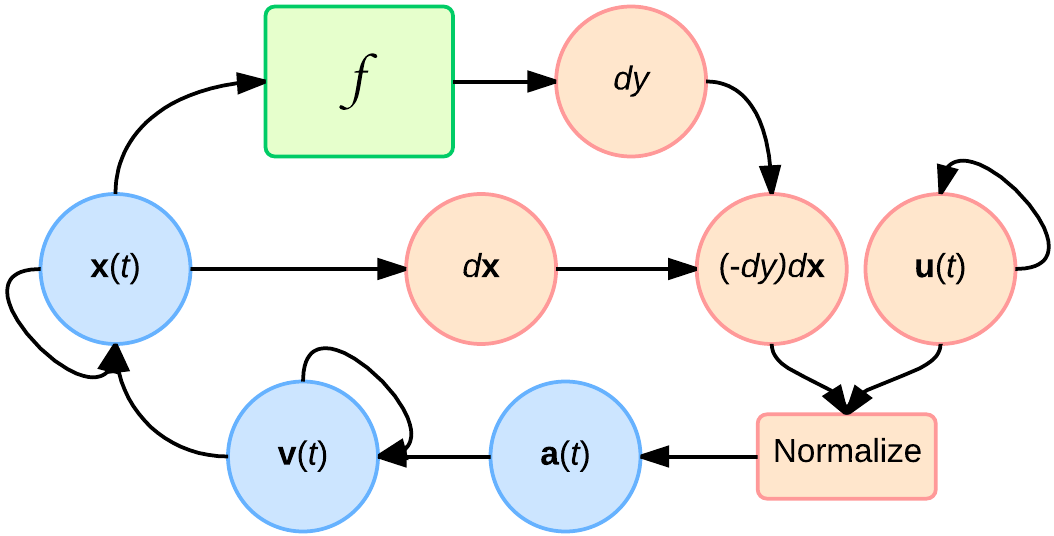
\includegraphics[width=0.5\textwidth]{hill_network.png}
  \caption{(Network Architecture) $\bolds{x}(t)$, $\bolds{v}(t)$, $\bolds{a}(t)$ are populations of neurons representing the input's position, velocity, and acceleration, respectively. $f$ is the arbitrary feed-forward network being optimized. Remaining nodes are signal operations implemented in Nengo.}
\end{figure}

An immediate problem is that, since $dy$ is a scalar, the error has no directional information apart from its sign. This causes $\bolds{x}(t)$ to oscillate back and forth along the line $\bolds{x}(0) + c \bolds{v}(0)$, $c \in \mathbb{R}$. 

A natural solution was to introduce periodic perturbations to the acceleration, in the form of a control $\bolds{u}(t)$ term. This term emits a pulse lasting 20ms that alternates every 200ms between different vectors taken from some arbitrarily chosen basis for $\mathbb{R}^d$, denoted $\mathcal{B}$.

In effect, $\bolds{x}(t)$ will move back and forth in one direction, while being periodically pushed in a new direction. Since $\mathcal{B}$ spans the vector space, it follows from standard results in linear algebra that this should converge to a local minimum, given appropriate scaling on $\bolds{v}(t)$ and $\bolds{a}(t)$\footnote{We scaled acceleration by $50$ and velocity by $5$}.

The basis $\mathcal{B}$ can be understood as encoding some prior knowledge, or {\it intuition}, about the problem. These vectors alter the trajectory, regardless of the state of $\bolds{x}$. If nothing is known about $f$, then we may let $\mathcal{B}$ be the canonical basis of $\mathbb{R}^d$, which reduces to testing rectilinearly adjacent points. However, if something is known about the directions that tend to minimize error, due to the structure of $f$, then it may be desirable to incorporate this knowledge into $\mathcal{B}$, in effect biasing the neighborhood of $\bolds{x}(t)$. Furthermore, since $\bolds{u}(t)$ merely perturbs the velocity relative to its current state, the neighbourhood's frame of reference will shift dynamically, an approach shared by dynamic hill climbing, which has the practical benefit of overcoming many common limitations of hill climbing \cite{yuret1993dynamic}.

Neurons encoding the position, velocity, and acceleration, were modeled using a Leaky-Integrate-and-Fire (LIF) circuit with an RC time constant of $\tau_{rc} = 20$ms and a refractory period of $\tau_{ref} = 2$ms.  

Due to time constraints, the differentiation, computation of $(-dy)d\bolds{x}$, and oscillatory behaviour of $\bolds{u}(t)$, were all implemented by directly manipulating the vectors, rather than by use of neural nonlinearities. Thus, the network is not biologically plausible in its current form\footnote{Post-synaptic filtering was still modeled by convolving the feedback signal with an exponential filter with decay $\tau = 5$ms}. However, previous work has demonstrated that differentiation, multiplication, and oscillations of specific frequencies, are all possible using spiking neurons and NEF methods \cite{tripp2010, huzook2012}.

%\begin{figure}[t] \label{fig-u}
%  \centering
%  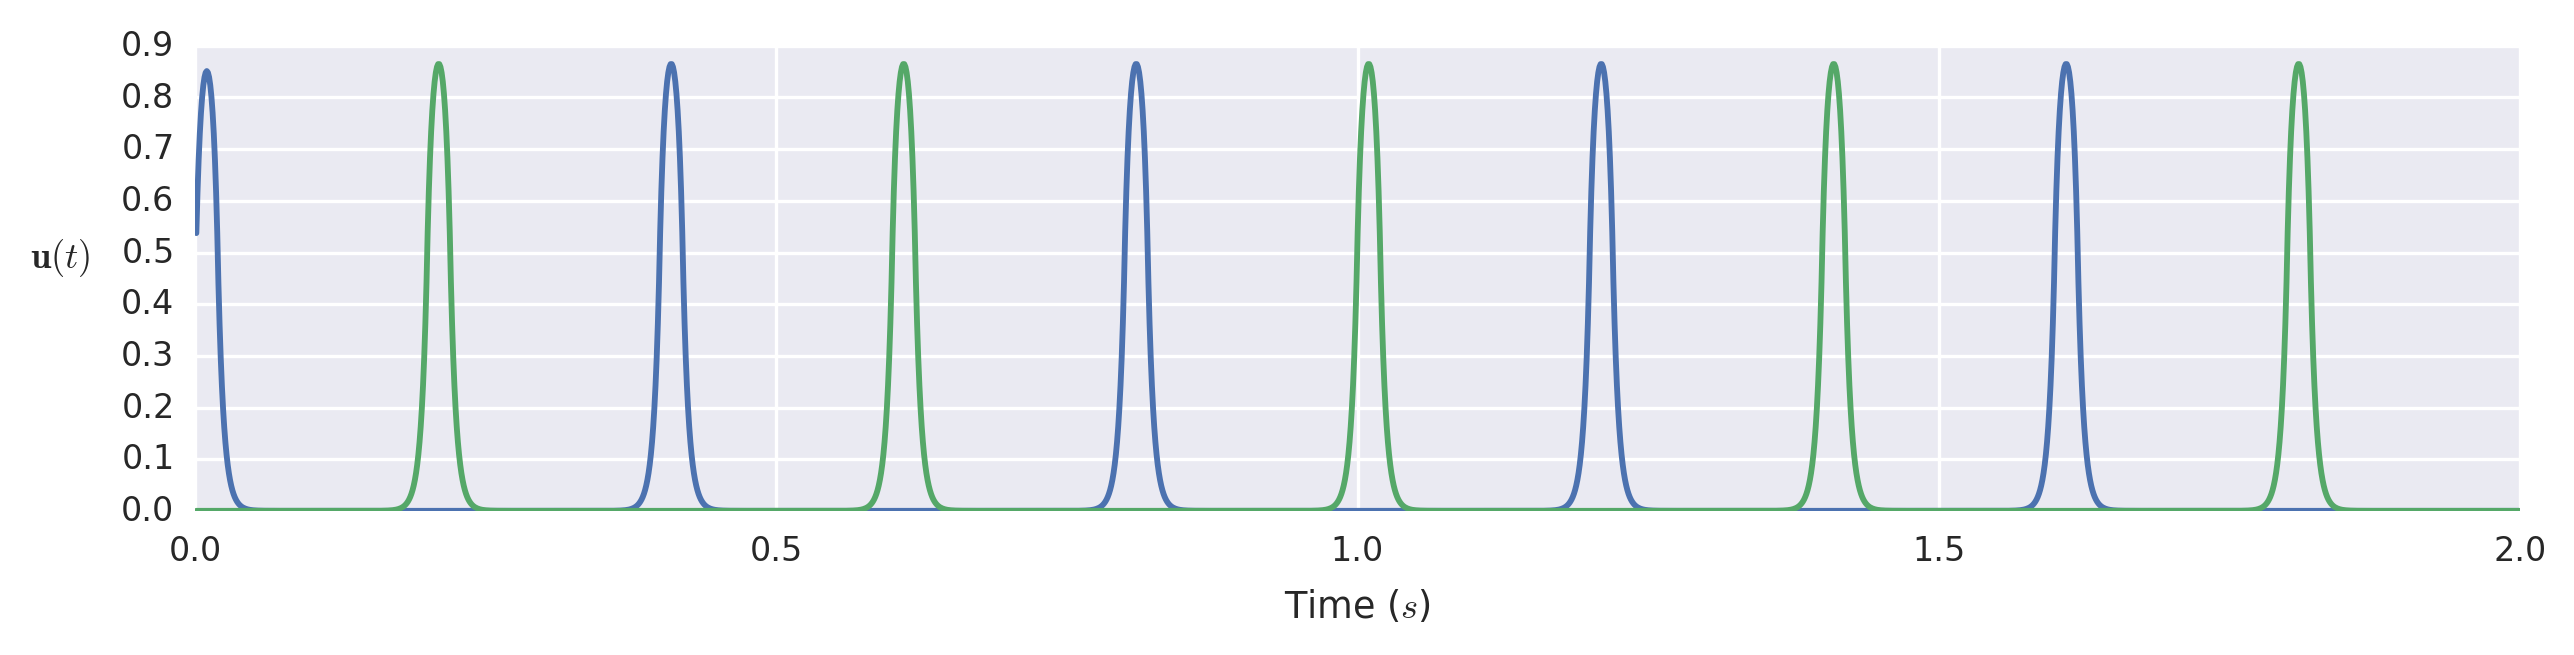
\includegraphics[width=0.5\textwidth]{u.png}
%  \caption{Two-dimensional $\bolds{u}(t)$ with axis-aligned basis vectors, %plotted over a $2$ second interval. Rise and decay times are the result of %post-synaptic filtering.}
%\end{figure}

\begin{figure*}[ht]
  \centering
  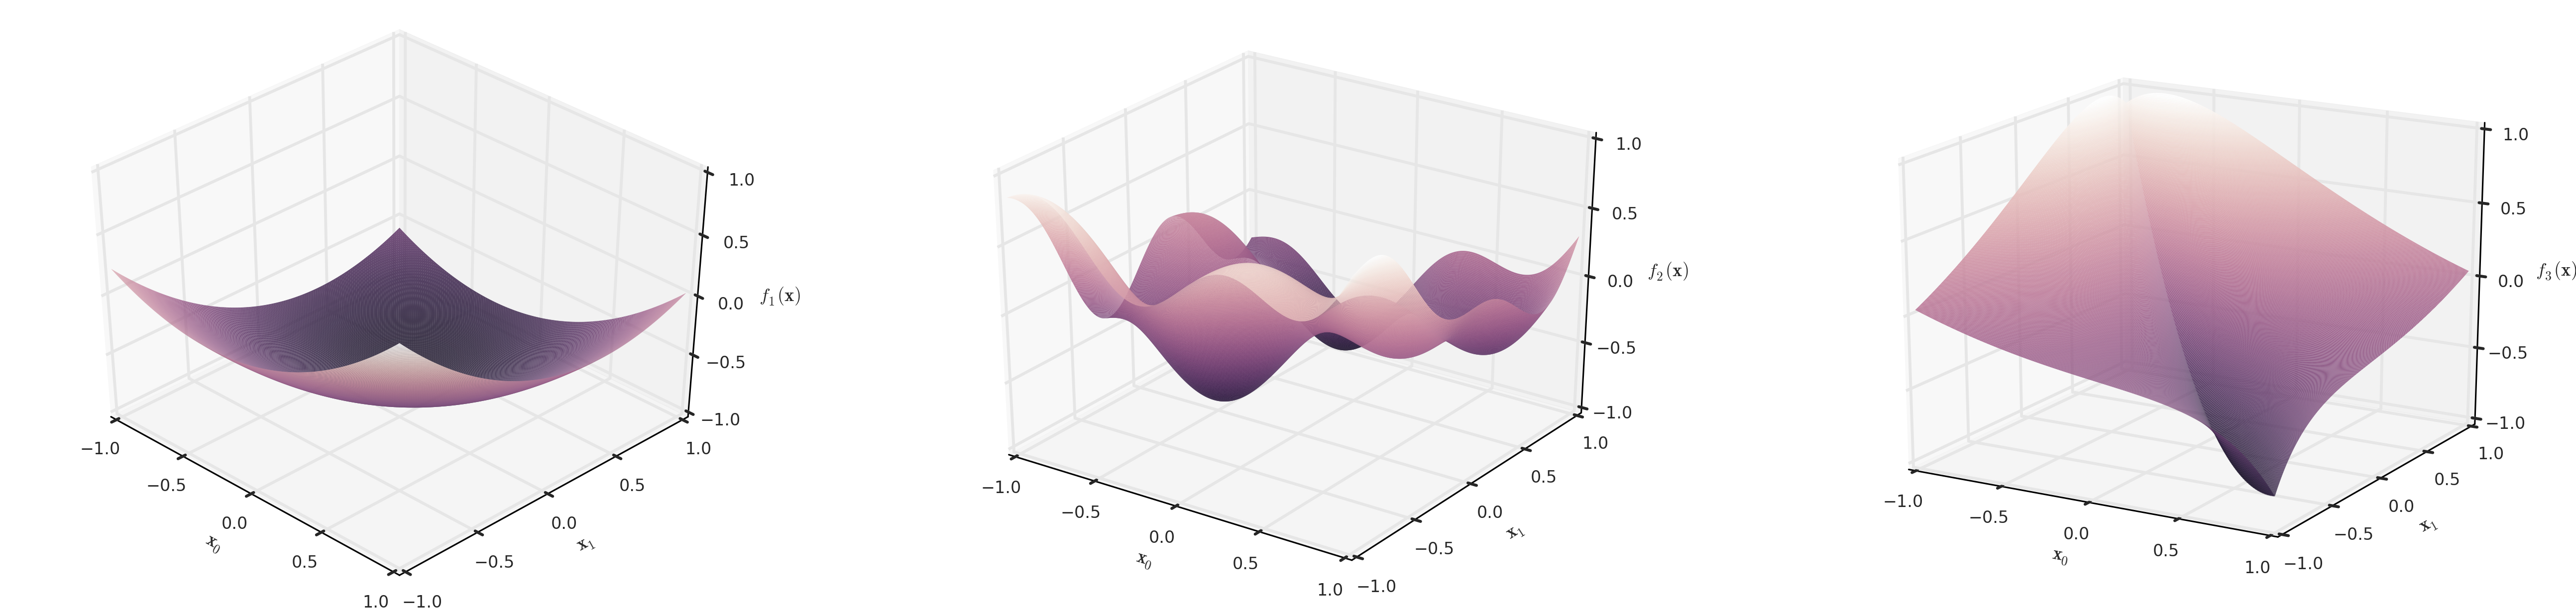
\includegraphics[width=1.0\textwidth]{functions.png}
  \caption{Surface plots of the three test functions, corresponding to equations \ref{eq-f1}, \ref{eq-f2}, \ref{eq-f3}, from left to right, respectively.}
\end{figure*}

\section{Neural Engineering Framework (NEF)}

The NEF is a set of biologically-motivated principles that provide methods for converting a mathematical description of a system (such as section \ref{sec-model}) into a network of spiking neurons. The following overview has been adapted from Stewart \cite{stewart2012b}, which may be consulted for further details.

The first principle gives us a way to represent a vector, $\bolds{x}$, in the spiking activity of a population of neurons. Each neuron $i$ has an {\it encoding vector}, $\bolds{e}_i$, which can be understood as the vector for which this neuron will fire most strongly. The principle states that the input current to the neural nonlinearity, $G$, is a linear function of $\bolds{x}$, with coefficients given by $\bolds{e}_i$, scaled by a gain of $\alpha_i$, plus a bias current $\beta_i$. This gives a concise equation for each neuron's activity:

\begin{equation} \label{eq-neuron}
a_i = G[\alpha_i \bolds{e}_i \cdot \bolds{x} + \beta_i]
\end{equation}

To decode the vector from this activity, we find a set of linear decoding weights $\bolds{d}$ for each neuron, to approximate

\begin{equation} \label{eq-decoder}
\bolds{x} \approx \sum_i a_i \bolds{d}_i.
\end{equation}

These weights can be found by optimizing a chosen error function. We typically minimize the root-mean-squared error using standard least squares solvers.

The second principle states that transformations of these vectors can be computed in the connection weights between populations of neurons. For instance, the connection weight from neuron $i$ to $j$ that computes the identity function is

\begin{equation}
\omega_{ij} = \bolds{d}_i \cdot \bolds{e}_j.
\end{equation}

Interestingly, the same equation can be used to approximate any arbitrary function, by modifying the optimization problem given by equation \ref{eq-decoder} to decode a function of \bolds{x}, i.e. by approximating $f(\bolds{x}) \approx \sum_i a_i \bolds{d}^{f}_i$.

The third principle provides a means for converting a control-theoretic description of a dynamical system into a recurrently connected population. For the purposes of this work, we are mainly interested in the simplest case of integrating an input vector:

\begin{equation} \label{eq-dynamics}
\frac{d\bolds{x}}{dt} = \bolds{u}.
\end{equation}

By using an exponential model to filter the post-synaptic current, $h(t) = e^{\frac{-t}{\tau}}$ (decay time constant $\tau$), it is easy to show that $\bolds{x}$ can be represented according to equation \ref{eq-dynamics} by setting the input to $\tau \bolds{u}$, with a recurrent transformation approximating the identity function \cite{conklin2005}.

\section{Results}

The model was built and simulated using Nengo \cite{bekolay2013nengo}, a software package for designing and simulating neural networks according to NEF principles. All figures and tables in this paper may be reproduced in full by running the Python code available on GitHub\footnote{\url{http://github.com/arvoelke/hill-climbing}}.

All simulations were performed on a conventional desktop computer\footnote{Intel\textregistered\enspace Core\texttrademark\enspace i7-4770 CPU @ 3.4GHz (64-bit)} with a simulation time step of 1ms and 1,000 neurons per population (3,000 total).

\begingroup\makeatletter\def\f@size{5}\check@mathfonts\def\maketag@@@#1{\hbox{\m@th\normalsize\normalfont#1}}%
\begin{align}%
\label{eq-f1} f_1(x_0, x_1) &= .5(x_0 + 0.3)^2 + .5(x_1 - 0.4)^2 - 1 \\
\label{eq-f2} f_2(x_0, x_1) &= .2\sin(6x_0) + .2\sin(6x_1) - .2\sin(2x_0)\sin(4x_1) \nonumber \\ & + .4(x_0 + 0.3)^2 + .4(x_1 - 0.5)^2 - .5 \\
\label{eq-f3} f_3(x_0, x_1) &= .7((.5(x_0 - x_1) - .6)^2 - e^{-3|x_0 + x_1|} - .3)
\end{align}
\endgroup

Three $2$-dimensional functions were considered: a convex bowl (equation \ref{eq-f1}), a sinusoidal function with multiple peaks and valleys (equation \ref{eq-f2}), and a narrow {\it ridge function} that cannot be optimized by standard hill climbing (equation \ref{eq-f3}). For convenience, each function is defined over the interval $[-1, 1]^2$ and normalized to the range $[-1, 1]$.

Simulations were run for 3 seconds (3,000 time steps), with each trial randomizing $\alpha_i$, $\beta_i$, $\bolds{e}_i$ for all neurons (equation \ref{eq-neuron}), and selecting a random set of basis vectors ($\mathcal{B}$). All model parameters, including the connection weights between neurons, were chosen independently of the particular function being optimized.

To quantitatively evaluate the algorithm, 100 trials were run on each function. Each trial recorded the best solution by decoding the neural activity (equation \ref{eq-decoder}). Accuracy was calculated by taking the difference between this best solution and the actual global minimum. We also reported the simulation time by determining which time step obtained the minimum. Means are summarized in table I, with standard deviations given in parentheses.

\begin{table}[h] \label{table-perf}
\captionof{table}{Model Performance}
\begin{center}
\begin{tabular}{|c|c|c|}
\hline
Function & Accuracy & Simulation Time ($s$) \\
\hline
$f_1$ & $0.0021$ $(\pm0.004)$ & $1.50s$ $(\pm0.9s)$ \\
$f_2$ & $0.0996$ $(\pm0.030)$ & $1.68s$ $(\pm0.9s)$ \\
$f_3$ & $0.0308$ $(\pm0.061)$ & $2.00s$ $(\pm0.8s)$ \\
\hline
\end{tabular}
\end{center}
\end{table}

%\addtolength{\textheight}{-2cm}   % This command serves to balance the column lengths
                                  % on the last page of the document manually. It shortens
                                  % the textheight of the last page by a suitable amount.
                                  % This command does not take effect until the next page
                                  % so it should come on the page before the last. Make
                                  % sure that you do not shorten the textheight too much.

\begin{figure}[tb!]
  \centering
  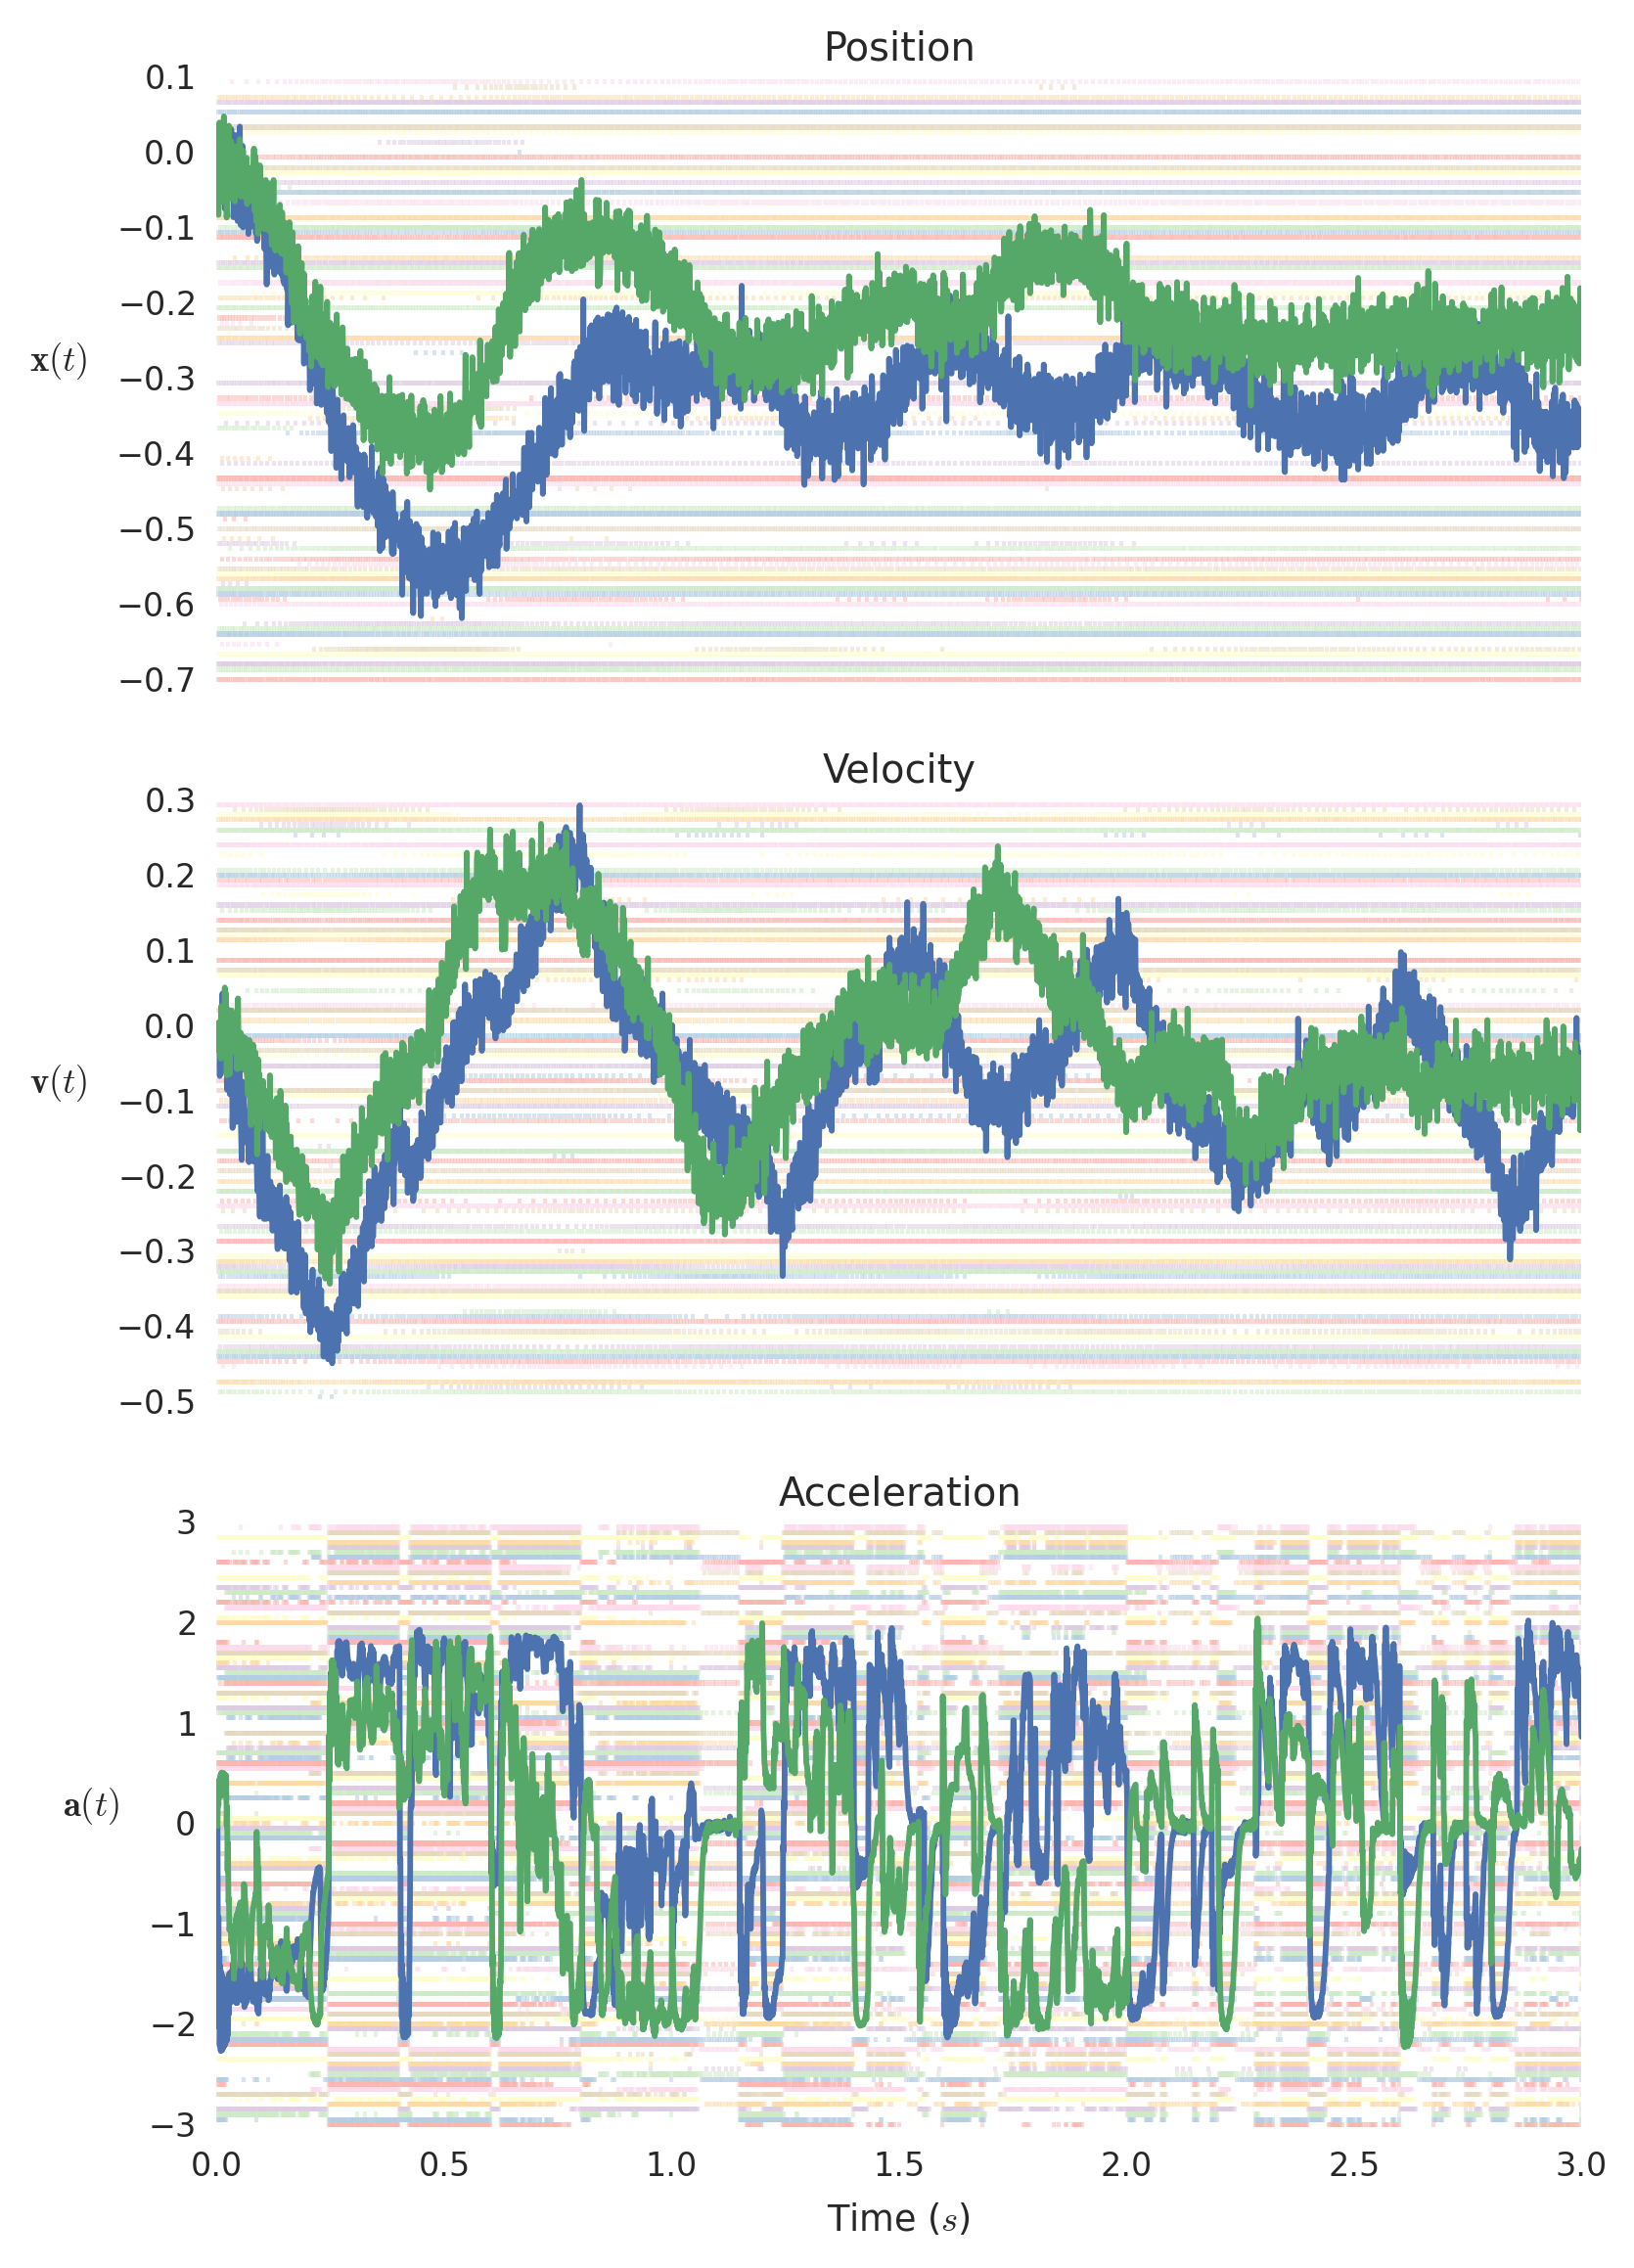
\includegraphics[width=0.5\textwidth]{probes.png}
  \caption{Simulation data from a randomly chosen trial on $f_2$. The decoded and filtered activity shows that all three populations oscillate while repeatedly crossing a local minimum. Spike rasters of 120 randomly chosen neurons, taken from each population, are rendered in the backgrounds of their respective plots.}
\end{figure}

\begin{figure*}[ht] \label{fig-paths}
  \centering
  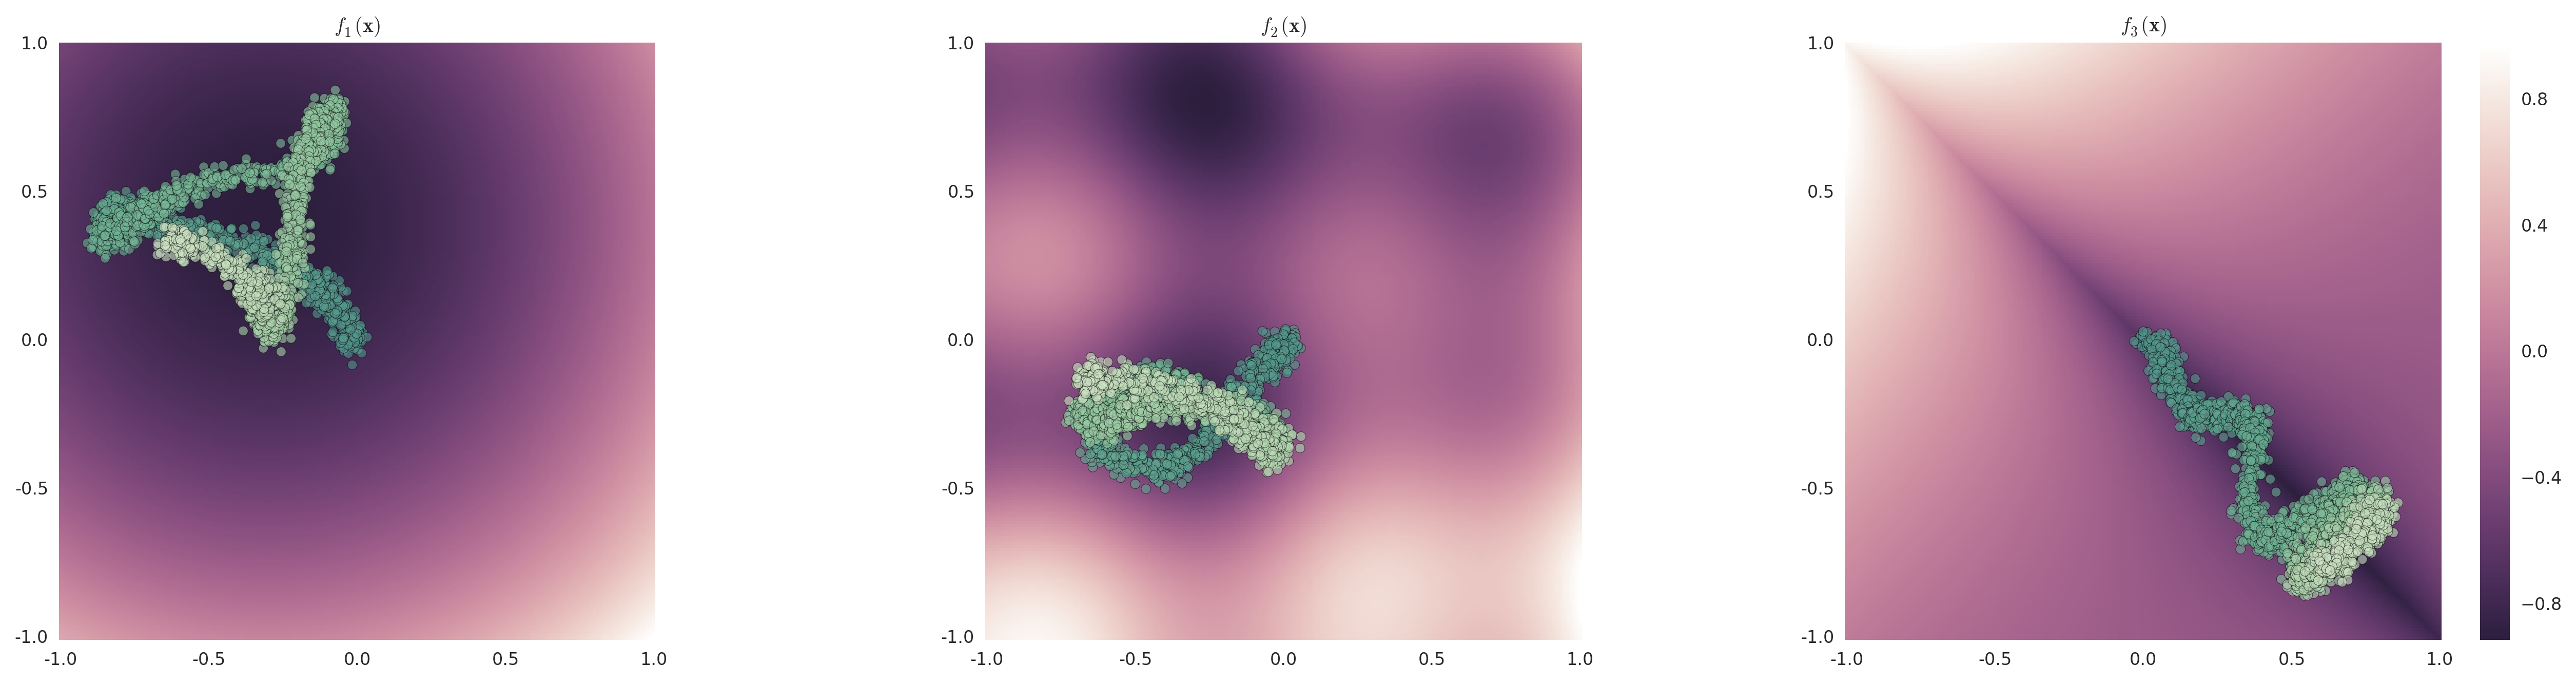
\includegraphics[width=1.0\textwidth]{paths.png}
  \caption{Selected simulation for each test function, with the decoded estimate for $\bolds{x}(t)$ overlaid to trace out the solution's path. (Left) The solution slowly circles around the minimum of $f_1$, since the region is convex with a gentle slope. (Center) The initial velocity sends $\bolds{x}(t)$ to the nearest (suboptimal) local minimum of $f_2$. The basis vectors are made visible by a distinctive ``X'' pattern, while the solution oscillates over the valley. (Right) The initial perturbation is not orthogonal to the ridge, and so the solution saddles toward the minimum of $f_3$. The firing rates of the LIF neurons saturate at the radius of the unit cicle, causing $\bolds{x}(t)$ to oscillate along the boundary.} % TODO: give a detailed account of the qualities going on here
\end{figure*}

\section{Conclusions}

\subsection{Discussion}

The results from table I demonstrate that this method performs well on the chosen test functions. In particular, the global optimum for $f_1$ is located almost perfectly with very little standard deviation. The error is largest for $f_2$, due to the existence of a suboptimal minimum close to $(0, 0)$.

%\begin{bottompar}
The high variability reflects a connection between $\bolds{u}(t)$ and the algorithm's behaviour. Depending on the direction of the perturbations ($\mathcal{B}$), the solution may tend toward a different local minimum. This is also why the simulation times are highly variable -- not all solutions follow the same path. 

Similarly for $f_3$, there is a small probability that the chosen basis vectors are mostly orthogonal to the ridge, resulting in premature convergence.
%\end{bottompar}

Data from these simulations also provide qualitative insights into the relationship between the basis vectors and the search path, that depend on the function being optimized.

In general, the dynamic nature of the method, resulting from periodic perturbations to the velocity and noisy neural representation, allows it to overcome some common limitations of hill climbing, by continually considering new directions and occasionally making locally suboptimal decisions.

%\FloatBarrier
We conclude that constraining the implementation to operate using brain-like principles provided a solution with desirable characteristics for certain functions.

\subsection{Limitations and Future Work}

The math from section \ref{sec-model} may also be used to implement a hill climbing algorithm without directly using Nengo or the NEF. It would be interesting to compare this approach with other hill climbing extensions on a standard suite of functions.  Likewise, the theoretical similarity between this approach and existing alternatives are not yet understood.

Limited analysis was performed on the effects of different basis vectors. Notably, greater performance may be achieved by allowing $\bolds{u}(t)$ to depend on the state of $\bolds{x}(t)$ and the magnitude of $dy$.

Currently, parts of the system are not biologically plausible. We believe this can be improved in future iterations of the model. More importantly, this work has not attempted to identify how the components of this system map onto neuroanatomically relevant brain regions. This undertaking would allow us to constrain the model using more detailed biological parameters and make specific predictions about what activity might be observed within these brain areas, during various cognitive tasks.

\section*{Acknowledgment}

Aaron Voelker would like to acknowledge both Chris Eliasmith and the Centre for Theoretical Neuroscience for establishing the positive environment which disseminated many of the ideas necessary for this work. We would also like to sincerely thank Gladimir Baranoski for inspiring this particular thread of research while lecturing for his course, {\it On the Synergy between Computer Science and Biology}, at the University of Waterloo.

\bibliographystyle{IEEEbib}
\bibliography{root}


\end{document}